\documentclass[tikz,border=10pt]{standalone}
\usepackage{tikz}
\usetikzlibrary{arrows.meta, positioning, calc, fit}

\begin{document}
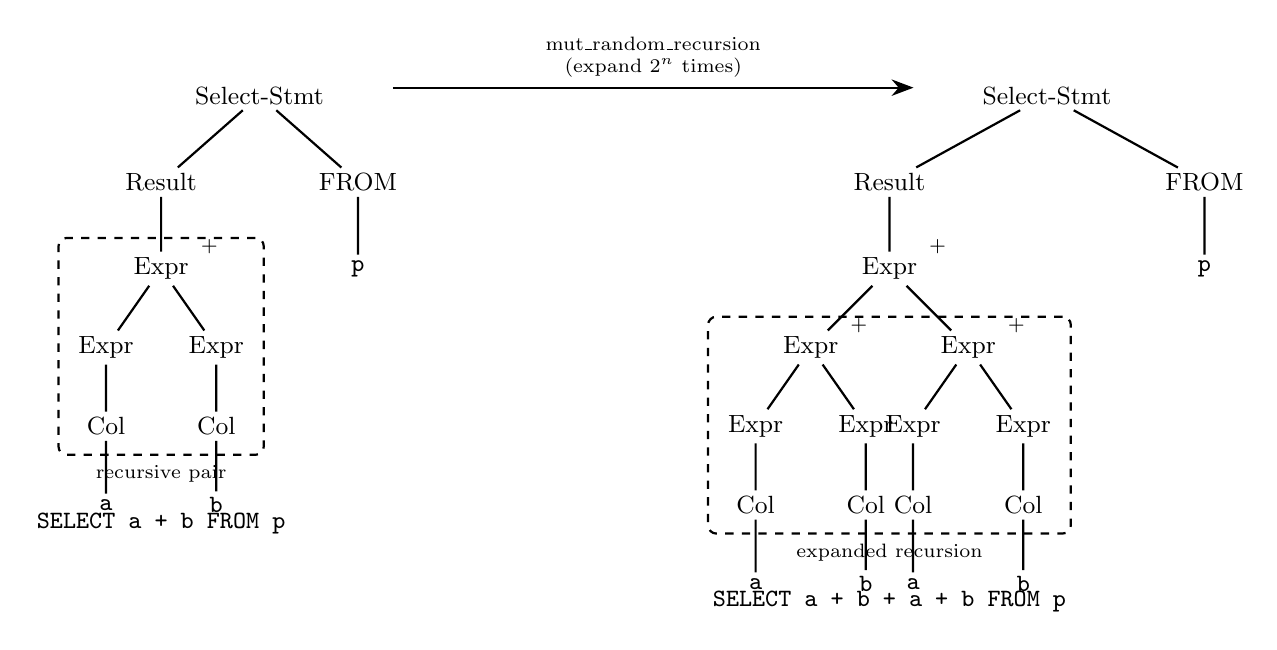
\begin{tikzpicture}[
    every node/.style={font=\small},
    tnode/.style={align=center, inner sep=2pt},
    oplab/.style={font=\scriptsize, inner sep=1pt},
    edge from parent/.style={draw, thick},
    arrow/.style={-{Stealth[scale=1.2]}, thick},
    dashrect/.style={draw, dashed, thick, rounded corners=3pt, inner sep=5pt},
    level 1/.style={sibling distance=2.5cm, level distance=1.1cm},
    level 2/.style={sibling distance=1.8cm, level distance=1.1cm},
    level 3/.style={sibling distance=1.4cm, level distance=1.0cm},
    level 4/.style={sibling distance=1.0cm, level distance=1.0cm},
    level 5/.style={sibling distance=1.0cm, level distance=1.0cm},
]

% ===== LEFT TREE (Before) =====
\node[tnode] (L-root) {Select-Stmt}
    child {node[tnode] (L-result) {Result}
        child {node[tnode] (L-expr) {Expr}
            child {node[tnode] (L-el) {Expr}
                child {node[tnode] (L-col-a) {Col}
                    child {node[tnode, font=\small\ttfamily] {a}}
                }
            }
            child {node[tnode] (L-er) {Expr}
                child {node[tnode] (L-col-b) {Col}
                    child {node[tnode, font=\small\ttfamily] {b}}
                }
            }
        }
    }
    child {node[tnode] (L-from) {FROM}
        child {node[tnode, font=\small\ttfamily] {p}}
    };

% Operator label
\node[oplab, above right=-2pt and 1pt of L-expr] {+};

% Dashed rectangle around recursive pair
\node[dashrect, fit=(L-expr)(L-el)(L-er)(L-col-a)(L-col-b),
      label={[font=\scriptsize, anchor=north]below:recursive pair}] (L-box) {};

% SQL label below
\node[below=0.6cm of L-box.south, font=\small\ttfamily, anchor=north] (L-sql)
    {SELECT a + b FROM p};


% ===== RIGHT TREE (After) =====
% Shift right for the expanded tree
\begin{scope}[xshift=10cm,
    level 1/.style={sibling distance=4.0cm, level distance=1.1cm},
    level 2/.style={sibling distance=3.2cm, level distance=1.1cm},
    level 3/.style={sibling distance=2.0cm, level distance=1.0cm},
    level 4/.style={sibling distance=1.4cm, level distance=1.0cm},
    level 5/.style={sibling distance=1.0cm, level distance=1.0cm},
    level 6/.style={sibling distance=1.0cm, level distance=1.0cm},
]
\node[tnode] (R-root) {Select-Stmt}
    child {node[tnode] (R-result) {Result}
        child {node[tnode] (R-top) {Expr}
            child {node[tnode] (R-left) {Expr}
                child {node[tnode] (R-ll) {Expr}
                    child {node[tnode] (R-col-a1) {Col}
                        child {node[tnode, font=\small\ttfamily] {a}}
                    }
                }
                child {node[tnode] (R-lr) {Expr}
                    child {node[tnode] (R-col-b1) {Col}
                        child {node[tnode, font=\small\ttfamily] {b}}
                    }
                }
            }
            child {node[tnode] (R-right) {Expr}
                child {node[tnode] (R-rl) {Expr}
                    child {node[tnode] (R-col-a2) {Col}
                        child {node[tnode, font=\small\ttfamily] {a}}
                    }
                }
                child {node[tnode] (R-rr) {Expr}
                    child {node[tnode] (R-col-b2) {Col}
                        child {node[tnode, font=\small\ttfamily] {b}}
                    }
                }
            }
        }
    }
    child {node[tnode] (R-from) {FROM}
        child {node[tnode, font=\small\ttfamily] {p}}
    };

% Operator labels
\node[oplab, above right=-2pt and 1pt of R-top] {+};
\node[oplab, above right=-2pt and 1pt of R-left] {+};
\node[oplab, above right=-2pt and 1pt of R-right] {+};

% Dashed rectangle around expanded nodes (new level of recursion)
\node[dashrect, fit=(R-left)(R-ll)(R-lr)(R-col-a1)(R-col-b1)(R-right)(R-rl)(R-rr)(R-col-a2)(R-col-b2),
      label={[font=\scriptsize, anchor=north]below:expanded recursion}] (R-box) {};

% SQL label below
\node[below=0.6cm of R-box.south, font=\small\ttfamily, anchor=north] (R-sql)
    {SELECT a + b + a + b FROM p};
\end{scope}

% ===== ARROW between trees =====
\draw[arrow] ([xshift=0.8cm, yshift=0.1cm]L-root.east)
    -- node[above, font=\scriptsize, align=center, text width=4cm]
    {mut\_random\_recursion\\(expand $2^n$ times)}
    ([xshift=-0.8cm, yshift=0.1cm]R-root.west);

\end{tikzpicture}
\end{document}
